\subsection{Overview}
Different from uninformed search and informed search. 
\begin{outline}
    \1 Uninformed search
        \2 use only information on \textbf{current path}, that is, from goal to fringe
    \1 Informed search
        \2 use also \textbf{heuristics}, that is, information about how close nodes on the fringe are to a goal
\end{outline}

\noindent
A heuristics is a function that estimates \textbf{how close a state is to a goal}, which needs \textbf{domain knowledge} \\

There is different heuristic function: manhattan distance, euclidean distance, ....

\subsection{Greedy search}
The difference between greedy search and uniformed search is \textbf{SELECT = "priority queue, order elements by $h(n)$}, which is called "Best-first search". \\
The difference between greedy search and uniformed cost-sensitive search is:
\begin{outline}
    \1 Greedy Search uses heuristic to order.
    \1 UCS uses accumulated cost to order.
\end{outline}

\noindent
Is it optimal? No, it just takes \textbf{the most obvious result} as next step, but may not be the best one. (Short-term vs. Long-term) Thus, the properties of greedy search is: (Time and space complexity is just badly-guide DFS)
\begin{outline}
    \1 Time complexity: $O(b^{m})$
        \2 with b: branching factor, m: maximum depth
    \1 Space complexity: $O(b^{m})$
        \2 with b: branching factor, m: maximum depth
    \1 Completeness: \textcolor{red}{no}, like badly DFS
    \1 Optimal: \textcolor{red}{no}, it just choose the most obvious result instead of the optimal one
\end{outline}

\subsection{Beam search}
A variant of \st{greedy search} and breadth-first search. It is similar to breadth-first, but only expend \emph{k} times \textbf{each tier}. First build the whole tier, then keep \emph{k} elements in frontier. The properties of beam search is:
\begin{outline}
    \1 Time complexity: \textcolor{red}{$O(k \times b \times s)$}
        \2 with k: hyperparameter, b: branching factor, s: shallowest-solution depth
    \1 Space complexity: \textcolor{red}{$O(k \times b)$}
        \2 with k: hyperparameter, s: shallowest-solution depth
    \1 Completeness: no, may drop the goal
    \1 Optimal: no, not completeness not even optimal
\end{outline}

\noindent
When k = 1, it is called \textbf{"Hill-Climbing search"}. \\

\subsection{Combination of UCS and Greedy Search}
As we known, UCS uses \textbf{path cost = "Backward cost" = $g(n)$} (Figure~\ref{usc_path_cost}), and Greedy search uses \textbf{heuristic = "Forward cost = $h(n)$} (Figure~\ref{greedy_search_heuristic}). And if we combine those two cost to estimate the quality of our current state: $f(n) = g(n) + h(n)$. The \textbf{SELECT = "priority queue, order elements by $f(n)$"} \\

\begin{figure}[htbp]
    \centering
    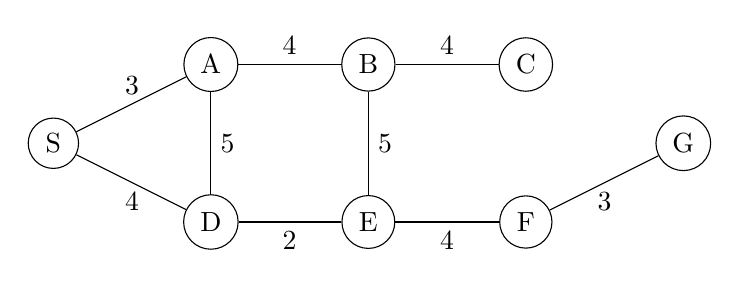
\begin{tikzpicture}
        \node [draw,circle](s)at(0,0){S};
        \node [draw,circle](a)at(2,1){A};
        \node [draw,circle](d)at(2,-1){D};
        \node [draw,circle](b)at(4,1){B};
        \node [draw,circle](e)at(4,-1){E};
        \node [draw,circle](c)at(6,1){C};
        \node [draw,circle](f)at(6,-1){F};
        \node [draw,circle](g)at(8,0){G};

        \draw (s) -- (a); 
        \draw (a) -- (b);
        \draw (b) -- (c);
        \draw (a) -- (d);
        \draw (s) -- (d);
        \draw (d) -- (e);
        \draw (b) -- (e);
        \draw (e) -- (f);
        \draw (f) -- (g);        

        \draw (1,1/2) node[above]{$3$};
        \draw (1,-1/2) node[below]{$4$};
        \draw (2,0) node[right]{$5$};
        \draw (3,1) node[above]{$4$};
        \draw (3,-1) node[below]{$2$};
        \draw (4,0) node[right]{$5$};
        \draw (5,1) node[above]{$4$};
        \draw (5,-1) node[below]{$4$};
        \draw (7,-1/2) node[below]{$3$};
    \end{tikzpicture}
    \caption{Path cost $g(n)$}
    \label{usc_path_cost}
\end{figure}

\begin{figure}[htbp]
    \centering
    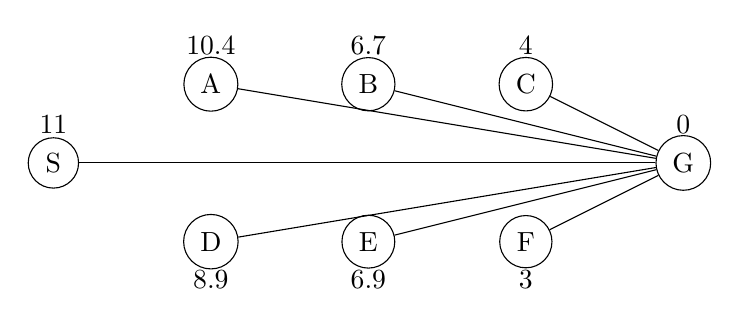
\begin{tikzpicture}
        \node [draw,circle](s)at(0,0){S};
        \node [draw,circle](a)at(2,1){A};
        \node [draw,circle](d)at(2,-1){D};
        \node [draw,circle](b)at(4,1){B};
        \node [draw,circle](e)at(4,-1){E};
        \node [draw,circle](c)at(6,1){C};
        \node [draw,circle](f)at(6,-1){F};
        \node [draw,circle](g)at(8,0){G};

        \draw (s) -- (g);
        \draw (a) -- (g);       
        \draw (d) -- (g);
        \draw (b) -- (g);
        \draw (e) -- (g);
        \draw (c) -- (g);
        \draw (f) -- (g);

        \draw (0,1/4) node[above]{$11$};
        \draw (2,5/4) node[above]{$10.4$};
        \draw (2,-5/4) node[below]{$8.9$};
        \draw (4,5/4) node[above]{$6.7$};
        \draw (4,-5/4) node[below]{$6.9$};
        \draw (6,5/4) node[above]{$4$};
        \draw (6,-5/4) node[below]{$3$};
        \draw (8,1/4) node[above]{$0$};
    \end{tikzpicture}
    \caption{Heuristic $h(n)$}
    \label{greedy_search_heuristic}
\end{figure}

\noindent
However, this is not enough for optimal. We need to do something on the heuristic cost. Otherwises, the actual bad goal cost < estimated good goal cost. \textbf{Admissible heuritics} is needed, they \textbf{underestimate the actual cost}. Saying that $h$ is admissible iff for all nodes $n \le h(n) \le h^{*}(n)$ where $h^{*}(n)$ is the actual cost to the closest goal. \\
How to come up with admissible heuristics? The cost of an optimal solution to a \textbf{relaxed problem} is admissible heuristics, an understimate, for the original problem. \\
Larger admissible heuristics, better estimation, closer to actual value, \textcolor{red}{but cannot larger than actual value (upper bound).} For example, $h2$ dominates $h1$ means for all nodes $n: h2(n) \ge h1(n)$. In this case, $h2$ is always better than $h1$, but for all nodes $h1(n) \le h2(n) \le h^{*}(n)$. For two heuristics $h1$ and $h2$, $h3(n) = max(h1(n),h2(n))$ always dominates both $h1$ and $h2$, because for all nodes n, $h3(n) \ge h1(n)$ and $h3(n) \ge h1(n)$.

\subsection{Summary}
\begin{enumerate}
    \item The best heuristics $f(n) = g(n) + h(n)$ is an \textbf{admissble heuristics} with the combination of Uniformed Cost Search and Greedy Search.
    \item Coming up with a good admissible heuristics is important (larger -> better -> closer to the $h^{*}(n)$ (actual value), but also should be (for all nodes n) smaller than $h^{*}(n)$)
\end{enumerate}

\pagebreak